\documentclass[a4paper]{ctexart}
\def\SpineW{2cm} % 书脊宽度
% 总宽度 = 21 + SpineW + 21
\usepackage[paperwidth=21cm, paperheight=29.7cm, margin=0pt]{geometry}
\usepackage{tikz, xcolor, xeCJK, contour, graphicx, fontspec, expl3, xparse}
\usetikzlibrary{calc, fadings, decorations.text, positioning}
% 图片搜索路径
\graphicspath{{images/}}

% 中文字体
\defaultfontfeatures{Path=./fonts/}
\setCJKmainfont{simsun.ttc}
\newCJKfontfamily\zhongsong{STZHONGS.TTF}
\newCJKfontfamily\dengxian{Deng.ttf}[BoldFont=Dengb.ttf]
\newCJKfontfamily\heavyfont{SourceHanSansCN-Heavy.otf}
\newCJKfontfamily\heit{simhei.ttf}

% 英文/数字字体
\setmainfont{Dengb.ttf}
\newfontfamily\timeseng{times.ttf}
\newfontfamily\fzhteng{FZHT.TTf}[FakeBold=4]

% 颜色
\definecolor{rup}{RGB}{222,128,116} % 人字纹上色
\definecolor{rud}{RGB}{213,109,98} % 人字纹下色

\definecolor{jks}{RGB}{124,162,149} % 封面第二色，书脊“……教科书”色
\definecolor{xiu}{RGB}{160,156,155} % 封面第四色，书脊“……修”色

\definecolor{yinshua}{RGB}{0,165,79} % “绿色印刷产品”色
\contourlength{0.5pt} % “绿色印刷产品”文字外部白纹宽度

\definecolor{tl}{RGB}{124,162,149} % 扉页顶端左色
\definecolor{tr}{RGB}{184,147,123} % 扉页顶端右色

% 审核标
\newcommand{\usethemered}{%
	\definecolor{inc}{RGB}{253,199,155}%
	\definecolor{outc}{RGB}{255,0,0}%
	\def\circleimage{bred.png}%
}
\newcommand{\usethemegreen}{%
	\definecolor{inc}{RGB}{205,229,192}%
	\definecolor{outc}{RGB}{97,150,90}%
	\def\circleimage{bgreen.png}%
}
%\usethemered % 使用红色标
\usethemegreen % 使用绿色标

% 封面左部渐变
\pgfdeclarehorizontalshading{leftshading}{2.6cm}{
	color(0cm)=(pgftransparent!0); 
	color(1.1cm)=(pgftransparent!0);  
	color(2.6cm)=(pgftransparent!100) 
}
\pgfdeclarefading{leftfading}{\pgfuseshading{leftshading}}

% 封面人字纹数据
\def\WO{7.4cm} % 宽
\def\HO{1.8cm} % 高   
\def\StepO{0.25cm} % 竖直距离
\def\rx{-7cm} % 人字纹下限

% 扉页人字纹数据
\def\WT{6.8cm} % 宽
\def\HT{1.8cm} % 高   
\def\StepT{0.25cm} % 竖直距离
\def\uheight{4} % 下侧人字纹高度 

\def\N{40} % 数量

% 数学版本
\newcommand{\ab}{%
	\definecolor{abcolor}{RGB}{247,148,60} % A版颜色
	\node[
	anchor=south east,
	inner sep=0pt,
	outer sep=0pt,
	text=abcolor,
	xshift=-1.5cm,
	yshift=1.5cm
	] at (21cm,-29.7cm) {%
		{\dengxianeng\fontsize{60pt}{60pt}\selectfont A}%
		\hspace{-0.05em}%
		{\heit\fontsize{30pt}{30pt}\selectfont 版}%
	};
}

\newcommand{\bbo}{%
	\definecolor{bbcolor1}{RGB}{255,255,255} % B版封面
	\node[
	anchor=south east,
	inner sep=0pt,
	outer sep=0pt,
	text=bbcolor1,
	opacity=0.5,
	xshift=-1.5cm,
	yshift=1.5cm
	] at (21cm,-29.7cm) {%
		{\fontsize{60pt}{60pt}\selectfont B}%
		\hspace{-0.05em}%
		{\heit\fontsize{30pt}{30pt}\selectfont 版}%
	};
}

\newcommand{\bbt}{%
	\definecolor{bbcolor2}{RGB}{247,148,60} % B版扉页
	\node[
	anchor=south east,
	inner sep=0pt,
	outer sep=0pt,
	text=bbcolor2,
	opacity=0.5,
	xshift=-1.5cm,
	yshift=1.5cm
	] at (21cm,-29.7cm) {%
		{\fontsize{60pt}{60pt}\selectfont B}%
		\hspace{-0.05em}%
		{\heit\fontsize{30pt}{30pt}\selectfont 版}%
	};
}

% 书籍信息
\newcommand{\DiBookSeries}{PUTONG GAOZHONG JIAOKESHU}
\newcommand{\DiSubject}{YUANSHEN}

% 书类
\newcommand{\BookSeriesText}{普通高中教科书}
% 书封
\newcommand{\BookSeriesSpacing}{0.25em}
\newcommand{\BookSeriesInline}{%
	\renewcommand{\CJKglue}{\hspace{\BookSeriesSpacing}}%
	\BookSeriesText
}
% 扉页
\newcommand{\TBookSeriesSpacing}{1em}
\newcommand{\TBookSeriesInline}{%
	\renewcommand{\CJKglue}{\hspace{\TBookSeriesSpacing}}%
	\BookSeriesText
}
% 书脊
\ExplSyntaxOn
\cs_new:Npn \BookSeriesSplit
{
	\tl_set:Nx \l_tmpa_tl { \BookSeriesText }
	\seq_clear:N \l_tmpa_seq
	\tl_map_inline:Nn \l_tmpa_tl
	{
		\seq_put_right:Nn \l_tmpa_seq { ##1 }
	}
	\seq_use:Nn \l_tmpa_seq { \\ }
}
\ExplSyntaxOff

\newcommand{\SubjectText}{原神} % 原始文本
\newcommand{\SubjectInline}{原神} % 封面
\newcommand{\SubjectFont}{75}
\newcommand{\SubjectSize}{75} 

\ExplSyntaxOn
\NewDocumentCommand{\SSubject}{ }
{
	\tl_set:Nx \l_tmpa_tl { \SubjectText } % 获取原始文本 
	\int_set:Nn \l_tmpa_int { \tl_count:N \l_tmpa_tl } % 计算总字数
	\int_zero:N \l_tmpb_int
	
	\tl_map_inline:Nn \l_tmpa_tl
	{
		\int_incr:N \l_tmpb_int
		##1 % 输出当前字符
		% 如果不是最后一个字，则插入 \hfill 和一个空格
		\int_compare:nT { \l_tmpb_int < \l_tmpa_int }
		{ \hfill{} } 
	}
} % 中学xx课程

\cs_new:Npn \SubjectSplit
{
	\tl_set:Nx \l_tmpa_tl { \SubjectText }
	\seq_clear:N \l_tmpa_seq
	\tl_map_inline:Nn \l_tmpa_tl
	{
		\seq_put_right:Nn \l_tmpa_seq { ##1 }
	}
	\seq_use:Nn \l_tmpa_seq { \\ }
}
\ExplSyntaxOff

\newcommand{\EditionText}{选修16}
\newcommand{\EditionSpacing}{0.5em}
\ExplSyntaxOn
\bool_new:N \l_last_was_num_bool % 记录上一个字符是否为数字
\bool_new:N \l_curr_is_num_bool  % 记录当前字符是否为数字

\NewDocumentCommand{\EditionInline}{ }
{
	\group_begin:
	\tl_set:NV \l_tmpa_tl \EditionText
	\int_set:Nn \l_tmpa_int { \tl_count:N \l_tmpa_tl }
	\int_zero:N \l_tmpb_int
	\bool_set_false:N \l_last_was_num_bool
	
	\tl_map_inline:Nn \l_tmpa_tl
	{
		\int_incr:N \l_tmpb_int
		\str_if_in:nnTF { 0123456789 } { ##1 }
		{ \bool_set_true:N \l_curr_is_num_bool }
		{ \bool_set_false:N \l_curr_is_num_bool }
		
		\int_compare:nT { \l_tmpb_int > 1 }
		{
			\bool_if:nTF { \l_last_was_num_bool && \l_curr_is_num_bool }
			{ } % 连续数字，不加间距
			{ \hspace{\EditionSpacing} } % 其他情况，加间距
		}
		
		% 3. 输出字符
		\bool_if:NTF \l_curr_is_num_bool
		{ \raisebox{0.1ex}{##1} }
		{ ##1 }
		
		% 4. 更新状态供下一轮使用
		\bool_set_eq:NN \l_last_was_num_bool \l_curr_is_num_bool
	}
	\group_end:
}
\cs_new:Npn \EditionSplit
{
	\tl_set:Nx \l_tmpa_tl { \EditionText }
	\bool_set_false:N \l_last_was_num_bool
	\int_zero:N \l_tmpb_int
	
	\tl_map_inline:Nn \l_tmpa_tl
	{
		\int_incr:N \l_tmpb_int
		% 1. 判定当前字符属性
		\str_if_in:nnTF { 0123456789 } { ##1 }
		{ \bool_set_true:N \l_curr_is_num_bool }
		{ \bool_set_false:N \l_curr_is_num_bool }
		
		% 2. 换行逻辑：只要不是 (上一个是数字 且 当前是数字)，就换行
		\int_compare:nT { \l_tmpb_int > 1 }
		{
			\bool_if:nTF { \l_last_was_num_bool && \l_curr_is_num_bool }
			{ 
				% 连续数字：只加一点极小的间距（可选），不换行
			}
			{ 
				\\ % 其他所有情况：强制换行
			}
		}
		
		% 3. 输出字符
		##1
		
		% 4. 关键：强制更新状态
		\bool_set_eq:NN \l_last_was_num_bool \l_curr_is_num_bool
	}
}
\ExplSyntaxOff

\newcommand{\ChapterText}{辞赋选读}
\newcommand{\ChapterColor}{black}
%\newcommand{\ChapterColor}{white}
\newcommand{\ChapterSpacing}{0.25em}
\newcommand{\ChapterInline}{%
	\renewcommand{\CJKglue}{\hspace{\ChapterSpacing}}%
	\ChapterText
}
\ExplSyntaxOn
\cs_new:Npn \__chapter_add_newline:n #1 { #1 \\ }

\cs_new:Npn \ChapterSplit
{
	\exp_args:No \tl_map_function:NN \ChapterText \__chapter_add_newline:n
}
\ExplSyntaxOff

% 审核标和奖标
\newcommand{\AuditText}{国家教材委员会专家委员会审核通过}
\newcommand{\YearText}{2026}
\newcommand{\PrizeText}{全国优秀教材一等奖}
\newcommand{\PrizeColor}{black}
%\newcommand{\PrizeColor}{white}

% 人教社颜色
\newcommand{\currentlogo}{rjsblack.png}
%\newcommand{\currentlogo}{rjswhite.png}

\newsavebox{\unitbox}
\savebox{\unitbox}{人民教育出版社\hspace{1em}课程教材研究所}
\newlength{\totalW}
\setlength{\totalW}{\wd\unitbox}
\def\lbj{14.3} % 编著信息左侧

\begin{document}
	\pagestyle{empty}

	\newlength{\MyBgWidth} % 背景图片宽度
	\setlength{\MyBgWidth}{\dimexpr 21cm + \SpineW + 2.6cm \relax}
	\pdfpagewidth=44cm \paperwidth=44cm	
	\begin{tikzpicture}[remember picture, overlay]
		\coordinate (BackNW) at (current page.north west); % 封底原点
		\coordinate (SpineNW) at ($(current page.north west) + (21cm, 0)$); % 书脊原点
		\coordinate (FrontNW) at ($(current page.north west) + (21cm + \SpineW, 0)$); % 封面原点
		
		% 封底
		\begin{scope}[shift={(BackNW)}]
			\begin{scope}[shift={(0, \rx)}]  
				\foreach \i in {\N, \numexpr\N-1\relax, ..., 0} {
					\pgfmathparse{mod(\i, 2) == 0 ? "rup" : "rud"}
					\let\currcolor\pgfmathresult
					\fill[\currcolor] 
					(0, \i*\StepO) 
					-- (0.5*\WO, \i*\StepO-\HO) 
					-- (\WO, \i*\StepO) 
					-- (1.5*\WO, \i*\StepO-\HO) 
					-- (2*\WO, \i*\StepO) 
					-- (2.5*\WO, \i*\StepO-\HO) 
					-- (3*\WO, \i*\StepO) 
					-- (3*\WO, -2) -- (0, -2) -- cycle;
				}
			\end{scope}
			
			\shade[path fading=south, fading angle=180, top color=rup!100!rud, bottom color=rup!0!rud] (0,\rx) rectangle (21cm, -1cm); % 人字纹渐变
			\fill[rup] (0, -1cm) rectangle (21cm, 0cm); % 人字纹上
			\fill[rud] (0, \rx) rectangle (21cm, -29.7cm); % 人字纹下  
			
			\node[anchor=south east, inner sep=0pt, outer sep=0pt] at (current page.south east) 
			{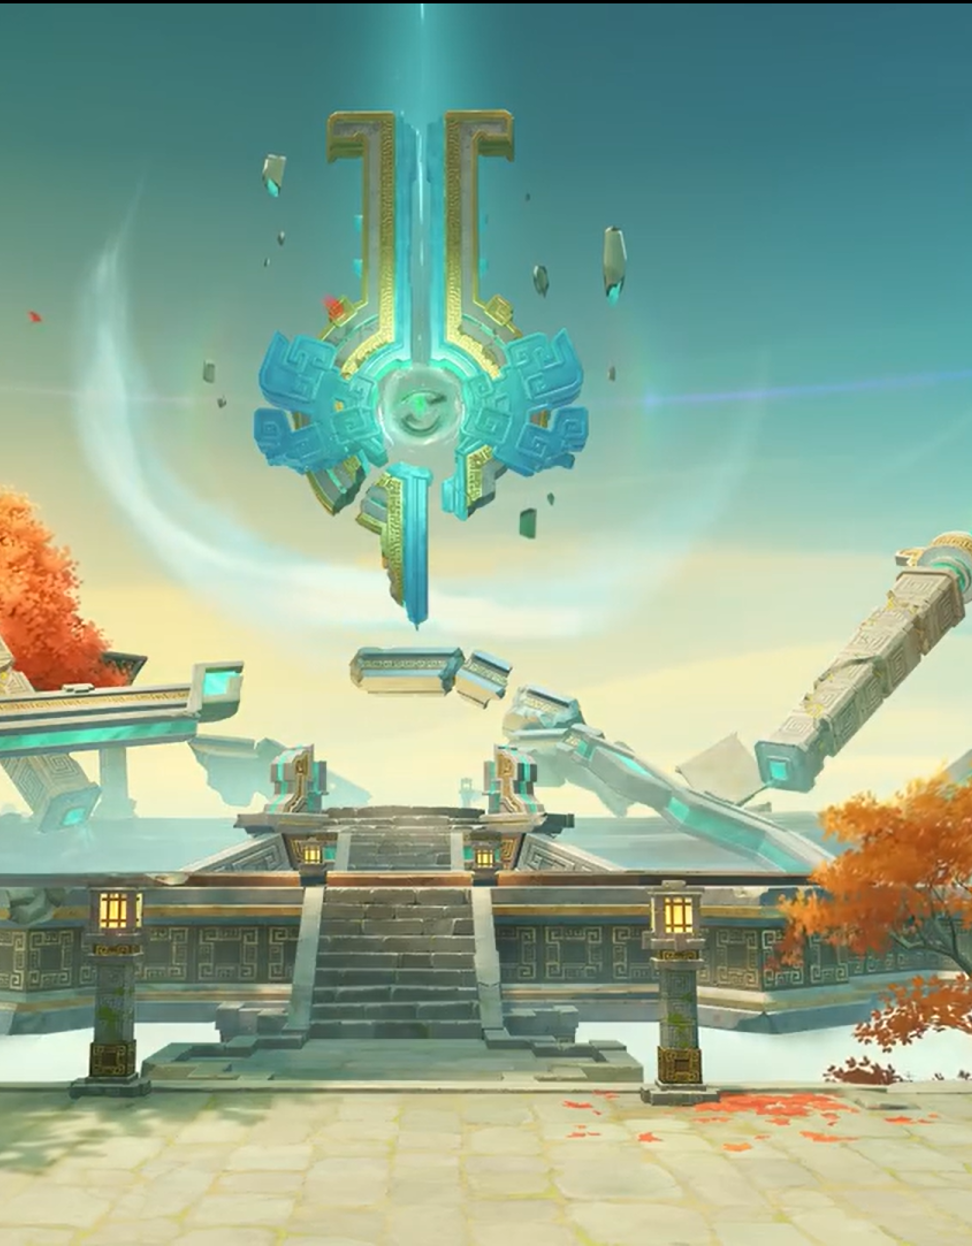
\includegraphics[width=\MyBgWidth, height=1.01\paperheight]{bg.png}}; % 背景图片
			
			\node[anchor=north west, inner sep=0pt, outer sep=0pt] 
			at ([shift={(0.7cm,-2cm)}]current page.north west) {
\includegraphics[width=2cm]{rjs.png}}; % 人教社标志
			
			\node[
			anchor=west,
			text=white,
			font=\Large,
			opacity=0.4
			] at ([shift={(0.7cm,2.9cm)}]current page.west) {\DiBookSeries};
			\node[
			anchor=west,
			text=white,
			font=\LARGE,
			opacity=0.4
			] at ([shift={(0.7cm,2cm)}]current page.west) {\DiSubject}; 
		
			\node[anchor=south west, inner sep=0pt, outer sep=0pt] 
			(img) at ([shift={(1cm,3cm)}]current page.south west) 
			{
\includegraphics[width=2.8cm]{hj.png}}; % 环境标志
			
			\node[anchor=north, font=\heit] 
			at (img.south) {\contour{white}{\textcolor{yinshua}{绿色印刷产品}}};
			
			\begin{scope}[shift={(21cm-2.6cm, 0)}]
				\foreach \col/\h [remember=\total as \total (initially 0)] in {rup/1, jks/6, rud/4.4, xiu/2.55} {
					\fill[\col] (0, -\total cm) rectangle (2.6 cm + \SpineW, -\total cm -\h cm);
					\pgfmathsetmacro{\total}{\total + \h}
				}
			\end{scope} % 封底右侧色块，延申及书脊
		
			\node[
			anchor=south east, 
			fill=white,             
			align=center,        
			font=\timeseng,
			inner sep=12pt
			] at ([shift={(-24.8cm,1.2cm)}]current page.south east) {
				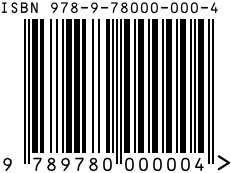
\includegraphics[width=3.2cm]{isbn.png}\\[0.15cm]
				\phantom{定价：20.23元}
			}; % 书籍信息
			
		\end{scope}
		
		% 书脊
		\begin{scope}[shift={(SpineNW)}]
			\tikzset{SpineNode/.style={
					inner sep=0pt,
					text width=\SpineW, % 使用书脊宽度作为盒子宽度
					align=center,       % 确保文本在盒子内部水平居中
					anchor=center
			}}
			
			\node[SpineNode, font=\large] at (\SpineW/2,-4cm) {\BookSeriesSplit};
			
			\node[SpineNode, font=\zhongsong\LARGE] at (\SpineW/2,-9.2cm) {\SubjectSplit}; 
			
			\node[SpineNode, font=\heit\large] at (\SpineW/2,-12.675cm) {\EditionSplit};
			
			\node[SpineNode, font=\zhongsong, text=\ChapterColor, anchor=north] at (\SpineW/2,-14.5cm) {\shortstack{\ChapterSplit}}; 
		\end{scope}
		
		% 封面
		\begin{scope}[shift={(FrontNW)}]
			\def\yd{-11.4} % 右侧参考点纵坐标			
			\begin{scope}
				\clip (12.85cm, \yd cm) rectangle (21cm, 0); % 剪切
				\begin{scope}[shift={(0, \rx)}]  
					\foreach \i in {\N, \numexpr\N-1\relax, ..., 0} {
						\pgfmathparse{mod(\i, 2) == 0 ? "rup" : "rud"}
						\let\currcolor\pgfmathresult
						\fill[\currcolor] 
						(0, \i*\StepO-\HO) 
						-- (0.5*\WO, \i*\StepO) 
						-- (\WO, \i*\StepO-\HO) 
						-- (1.5*\WO, \i*\StepO) 
						-- (2*\WO, \i*\StepO-\HO) 
						-- (2.5*\WO, \i*\StepO) 
						-- (3*\WO, \i*\StepO-\HO) 
						-- (3*\WO, -2) -- (0, -2) -- cycle;
					}				 
				\end{scope}
				\shade[path fading=south, fading angle=180, top color=rup!100!rud, bottom color=rup!0!rud] (0,\rx) rectangle (21cm, -1cm); % 人字纹渐变
				\fill[rup] (0, -1cm) rectangle (21cm, 0cm); % 人字纹上
				\fill[rud] (0, \rx) rectangle (21cm, -29.7cm); % 人字纹下 
			\end{scope}
			
			\node[
			anchor=east,
			font=\fontsize{14pt}{14pt}\selectfont,
			text=black,
			inner sep=0pt, 
			outer sep=0pt
			] at (18.55, -2.8) {\BookSeriesInline};
			
			\pgfmathsetmacro{\Height}{abs(\yd) - 5.05}
			\node[
			fill=white,
			anchor=north west,
			minimum width=6.35cm,
			minimum height=\Height cm,
			inner sep=0pt, 
			outer sep=0pt
			](mybox) at (12.85,-5.05) {};
			
			\begin{scope}[shift={(12.85cm, \yd cm)}]
			% 科目
%			\node[anchor=center, inner sep=0pt, outer sep=0pt, align=center, font=\zhongsong\fontsize{\SubjectFont pt}{\SubjectFont pt}\selectfont] at (mybox.center) {\SubjectInline};
			
			\node[ anchor=south west, inner sep=0pt, outer sep=0pt] at (0, 0) {
\includegraphics[width=6.35cm]{title.png}};
			
			\node[
			anchor=center,
			font=\LARGE\heit,
			text=gray,
			yshift=-2.4cm,
			inner sep=0pt,   
			outer sep=0pt,
			] at (mybox.center) {\EditionInline};
			
			\node[
			anchor=north west,
			fill=xiu,
			minimum width=6.35cm,
			minimum height=2.55cm,
			font=\zhongsong\Huge,
			inner sep=0pt,
			outer sep=0pt
			] at (0, 0) {\ChapterInline}; 
			\end{scope}
			
			\foreach \col/\h [remember=\total as \total (initially 0)] in {rup/1, jks/6, rud/4.4, xiu/2.55} {
				\fill[\col, path fading=leftfading] (0, -\total cm) rectangle (2.6cm, -\total cm -\h cm);
				\pgfmathsetmacro{\total}{\total + \h}
			}
			
			\coordinate (circleCenter) at (2.6cm, -2.5cm);
			\fill[white] (circleCenter) circle (1.5cm);
			%\node at (circleCenter) {
\includegraphics[width=3cm]{bz.png}};
			
			% 画的图片
			\fill[outc, even odd rule] (circleCenter) circle (1.45cm) (circleCenter) circle (1cm); % 圆环色
			\fill[inc] (circleCenter) circle (0.95cm); % 圆内色		
			\node[yshift=0.1cm] at (circleCenter) {\includegraphics[width=1.8cm]{\circleimage}};	
			
			\path[decoration={text along path, text={|\heavyfont\color{white}|\AuditText}, text align={fit to path}, raise=-2.3ex}, decorate] (circleCenter) ++(225:1.5cm) arc[start angle=225, end angle=-45, radius=1.5cm];
			\path[decoration={text along path, text={|\fzhteng|\YearText}, text align={fit to path}, raise=0.8ex}, decorate] (circleCenter) ++(250:1.5cm) arc[start angle=250, end angle=295, radius=1.5cm];
			
%			\coordinate (prizePos) at ($(circleCenter)+(3.5cm,0)$);
%			\node(prizeNode) at (prizePos) {
\includegraphics[width=3cm]{prize.png}};
%			\node[below=0.2cm of prizeNode] {\heit\textcolor{\PrizeColor}{\PrizeText}};
		
			\node[anchor=south west, xshift=2cm, yshift=1.5cm] 
			at (0,-29.7cm) {\includegraphics[width=6cm]{\currentlogo}};
			
			\bbo
		\end{scope}
	\end{tikzpicture}
	\clearpage
	\pdfpagewidth=21cm \paperwidth=21cm
	\begin{tikzpicture}[remember picture, overlay]
		\begin{scope}[shift={(current page.north west)}]
			\fill[tl] (0,0) rectangle (10.5, -1.2); % 顶端左
			\fill[tr] (10.5, 0) rectangle (21, -1.2); % 顶端右
			
			\begin{scope}
				\clip (0, -5.2) rectangle (21, -1.2);
				\begin{scope}[yshift=-5.2cm]
					\foreach \i in {\N, \numexpr\N-1\relax, ..., 0} {
						\pgfmathparse{mod(\i, 2) == 0 ? "rup" : "rud"}
						\let\currcolor\pgfmathresult
						\fill[\currcolor] 
						(0, \i*\StepT-\HT) 
						-- (0.5*\WT, \i*\StepT) 
						-- (\WT, \i*\StepT-\HT) 
						-- (1.5*\WT, \i*\StepT) 
						-- (2*\WT, \i*\StepT-\HT) 
						-- (2.5*\WT, \i*\StepT) 
						-- (3*\WT, \i*\StepT-\HT) 
						-- (3.5*\WT, \i*\StepT)
						-- (4*\WT, \i*\StepT-\HT)
						-- (4.5*\WT, \i*\StepT)
						-- (4.5*\WT, -2) -- (0, -2) -- cycle;
					}
				\end{scope}
				\shade[path fading=south, fading angle=180, 
				top color=rup!10!rud, bottom color=rup!0!rud] 
				(0, -5.2) rectangle (21, -1.2);
			\end{scope} % 上人字纹
			\fill[rud] (0, -5.2) rectangle (21cm, -8.2cm); % 中间过渡区
			
			\pgfmathsetmacro{\totalshift}{-8.2 - \uheight}
			\begin{scope}
				\clip (0, {-8.2-\uheight}) rectangle (21, -8.2);
				\begin{scope}[yshift=\totalshift cm]
					\foreach \i in {\N, \numexpr\N-1\relax, ..., 0} {
						\pgfmathparse{mod(\i, 2) == 0 ? "rud" : "rud!90!white"}
						\let\currcolor\pgfmathresult
						\fill[\currcolor] 
						(0, \i*\StepT) 
						-- (0.5*\WT, \i*\StepT-\HT) 
						-- (\WT, \i*\StepT) 
						-- (1.5*\WT, \i*\StepT-\HT) 
						-- (2*\WT, \i*\StepT) 
						-- (2.5*\WT, \i*\StepT-\HT) 
						-- (3*\WT, \i*\StepT) 
						-- (3.5*\WT, \i*\StepT-\HT)
						-- (4*\WT, \i*\StepT)
						-- (4.5*\WT, \i*\StepT-\HT)
						-- (4.5*\WT, -2) -- (0, -2) -- cycle;
					}
				\end{scope}
				\shade[path fading=south, fading angle=180, 
				top color=rud!90!white, bottom color=rud!0!white] 
				(0, -8.2) rectangle (21, -8.2-\uheight);
			\end{scope} % 下人字纹
			
			\node[anchor=center, font=\large] at (6,-5.7) {\TBookSeriesInline}; 
			
			\fill[white] (10.5,-1.2) rectangle (19.5,-8.5-\uheight); % 右侧白色
			
			%			\node[anchor=center, font=\zhongsong\fontsize{\SubjectSize pt}{\SubjectSize pt}\selectfont] at (15,-5.7) {\SubjectInline}; 
			
			\node[
			anchor=center,
			inner sep=0pt,
			outer sep=0pt
			] at (15, -5.7) {
\includegraphics[width=7cm]{title.png}};
			
			\node[anchor=center, font=\heit\LARGE, text=gray] at (15,-9.5) {
				{\EditionInline}
			}; 
			
			\node[anchor=center, font=\zhongsong\huge] at (15,-11.2) {\ChapterInline}; 
			
			\draw[black] (12.5,-10.2) -- (17.5,-10.2);
			\draw[black] (12.5,-12.2) -- (17.5,-12.2);
			
			
			\node[inner ysep=0pt] (line1) at (\lbj, -13.7) {\usebox{\unitbox}};
			\node[inner ysep=0pt] (line2) at (\lbj, -14.4) {%
				\makebox[\totalW][s]{中\hfill 学\hfill \SSubject\hfill 课\hfill 程\hfill 教\hfill 材\hfill 研\hfill 究\hfill 开\hfill 发\hfill 中\hfill 心}%
			};
			
			\coordinate (R) at ([xshift=0.1cm]line1.east);
			\coordinate (topR) at (R |- line1.north);
			\coordinate (bottomR) at (R |- line2.south);
			
			\coordinate (midR) at ($(topR)!0.5!(bottomR)$);
			\node[right, inner sep=5pt] (bz) at (midR) {编著};
			
			\draw (topR) -- (bottomR);
			\draw (bz.east |- line1.north) -- (bz.east |- line2.south);
			
			%\node[anchor=south] at (15, -13.7) {教育部组织编写};
			
			\node[anchor=center] at (10.5cm, -26.5cm) {
\includegraphics[width=5cm]{rjsblack.png}};
			
			\node[anchor=center] at (10.5cm, -27.3cm) {·北京·};
			
			\bbt
		\end{scope}
	\end{tikzpicture}
\end{document}